\section{Methods Affine}
We used the implemented affine registration from the MIA pipeline. To get the optimal we implemented a basic grid search. We tested 6 different parameters, which we thought to have the most influence on the registration accuracy. Because there is also a difference between on the result between different patients we tested each parameter combination with ten patients. \\ We registered the naive image to the mni image of the same patient. The pseudocode how we implemented the gridsearch can be seen in figure ~\ref{fig:pseudocode_gridsearch}. To evalutate the registration we calculated the dice.

\begin{figure}[!h]
	\centering
	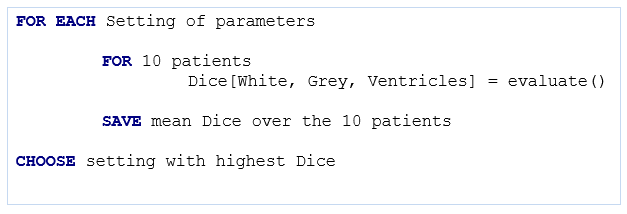
\includegraphics[width=2.5in]{pseudocode}
	% where an .eps filename suffix will be assumed under latex, 
	% and a .pdf suffix will be assumed for pdflatex; or what has been declared
	% via \DeclareGraphicsExtensions.
	\caption{The pseudocode how we implemented the grid search.}
	\label{fig:pseudocode_gridsearch}
\end{figure}
